
%%%%%%%%%%%%%%%%%%%%%%%%%%%%%%%%%%%%%%%%%%%%%%%%%%%%%%%%%%%%%%%%%%%%%%%%%%
Take a standard deck of 52 cards, with 13 $\spadesuit$, 13 $\heartsuit$, 13 $\diamondsuit$, and 13~$\clubsuit$. Shuffle it (well), so that the order is completely (uniformly)\footnote{People usually say ``random'' when they mean \emph{uniformly} random, and that can be quite ambiguous. I'll try not to.} random. \emph{How many consecutive pairs of the same suit do you expect?}

\begin{comment}
deck = StringJoin@*Reverse /@ 
  Tuples[{{"$\[SpadeSuit]$", "$\[HeartSuit]$", "$\[DiamondSuit]$", 
     "$\ClubSuit$"}, 
    Join[{"A"}, ToString /@ Range[2, 10], {"J", "Q", "K"}]}]
ResourceFunction["Shuffle"]["RandomSample"][deck]
\end{comment}

For instance,
\begin{center}
4$\heartsuit$, 3$\heartsuit$, 8$\clubsuit$, 2$\clubsuit$, 3$\spadesuit$, 10$\heartsuit$, 8$\diamondsuit$, 7$\spadesuit$, K$\heartsuit$, 5$\diamondsuit$, 8$\heartsuit$, J$\heartsuit$, 9$\clubsuit$, \\
5$\clubsuit$, J$\spadesuit$, 2$\heartsuit$, Q$\spadesuit$, 2$\spadesuit$, 10$\spadesuit$, 6$\spadesuit$, 6$\clubsuit$, 5$\heartsuit$, 4$\clubsuit$,  9$\spadesuit$,  Q$\diamondsuit$,  8$\spadesuit$,  \\
6$\diamondsuit$, 10$\diamondsuit$, 7$\clubsuit$, J$\clubsuit$, K$\clubsuit$, 4$\diamondsuit$, K$\diamondsuit$, K$\spadesuit$, A$\diamondsuit$, A$\spadesuit$, A$\clubsuit$, 4$\spadesuit$, A$\heartsuit$,  \\
3$\clubsuit$, 9$\diamondsuit$, 3$\diamondsuit$, J$\diamondsuit$, 9$\heartsuit$, Q$\heartsuit$, Q$\clubsuit$, 2$\diamondsuit$, 10$\clubsuit$, 5$\spadesuit$, 7$\diamondsuit$, 6$\heartsuit$, 7$\heartsuit$
\end{center}
has 15 such consecutive pairs.\marginnote{Please check.}

So\dots what's the expected number of consecutive same-suit pairs in a shuffled deck?

Let's try to estimate this:
\begin{lstlisting}
import numpy as np
import random
deck = 13*['S', 'H', 'D', 'C']
consecutives = []
for _ in range(50000):
    shuffled_deck = random.sample(deck, len(deck));
    consecutives += [np.sum([shuffled_deck[i] == shuffled_deck[i+1] for i in range(len(deck)-1)])]
print("Empirical mean: %f" % np.mean(consecutives))
\end{lstlisting}
I ran it: this gave $11.98176$. I ran it again: $12.0022$. And these 50,000 attempts look roughly like this (\cref{fig:consecutives}):
\begin{lstlisting}
import matplotlib.pyplot as plt
plt.hist(consecutives, density = True, bins=25, edgecolor='k');
plt.axvline(np.mean(consecutives), color='r', linestyle='dashed', linewidth=2)
plt.show()
\end{lstlisting}
\begin{figure}[htbp]\centering
    \label{fig:consecutives}
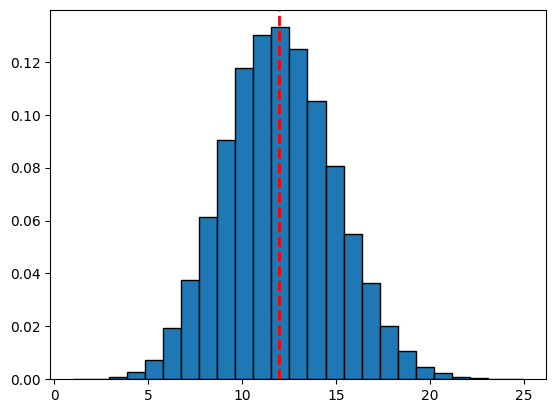
\includegraphics[width=0.7\textwidth]{figures/fig-consecutives-shuffled.png}
\caption{(Normalized) histogram of the number of consecutive pairs of the same suit, over $50,000$ trials. The red dashed line is the empirical mean.}
\end{figure}
Looks like this expected number is something like 12.\marginnote{Try to see what changes if you change the number of cards in the deck (for instance, 34 cards from each suit instead of 13). Could you have predicted it?} How do we explain this?

\begin{theorem}
    The expected number of consecutive same-suit pairs is 12.
\end{theorem}
\begin{proof}
    ``Linearity of expectation.''\marginnote{$\forall i$, $\probaOf{X_i = X_{i+1}} = \frac{13-1}{52-1}$}
\end{proof}

\subsection{One for the rainy days.} It's raining, and all $n$ students of the class come to the lecture with an umbrella. They all leave it in front of the lecture hall. At the end of the lecture, they leave the room in (uniformly) random order, and crossing the door each takes the closest remaining umbrella. In expectation, \emph{how many leave with their own umbrella}?

\begin{theorem}
    The expected number of fixed points in a uniformly random permutation of $\{1,2\dots,n\}$ is one.
\end{theorem}

%%%%%%%%%%%%%%%%%%%%%%%%%%%%%%%%%%%%%%%%%%%%%%%%%%%%%%%%%%%%%%%%%%%%%%%%%%
\section{What's a randomized algorithm?}
Randomized algorithms are algorithms whose behaviour \emph{does not
depend solely on the input.} It also depends (in part) on random
choices or the values of a number of \emph{random bits}.\smallskip

So we can think of the algorithm $\Algo$ as taking an input $x$ and a string of uniformly random bits $R\in\bool^\ast$. Now, since $\Algo$ is randomised, this could mean several things:
\begin{enumerate}
    \item The time $\tau_{\Algo}(x; R)$ that $\Algo$ takes on input $x$ is itself random, and depends on the random bits $R$
    \item The output $\Algo(x;R)$ of $\Algo$ on input $x$ is random, and can be different based on the random bits $R$
    \item Something else (\eg the amount of memory used by $\Algo$ could depend on the random bits)
    \item all, or any combination of the above
\end{enumerate}

Typically, what we want is then analyze $\Algo$ on \emph{worst-case} input $x$ and \emph{uniformly random} $R$. The two things to keep in mind: (1)~is the output of $\Algo$ always correct? Is it correct with high probability (over the choice of random bits $R$)? (2)~is the running time of $\Algo$ always bounded? Is it bounded with high probability, or in expectation (over the choice of random bits $R$)?\marginnote{\advancedstuff{} For those interested, for decision problems this is related to complexity classes \textsf{ZPP}, \textsf{RP}, and \textsf{BPP}. Think of that last one as ``randomized \textsf{P}.''}

\begin{description}
    \item[Las Vegas algorithms:] the algorithm is \emph{always correct}, but the running time is only bounded \emph{in expectation}. 
    \item[Monte-Carlo algorithms:] the algorithm is only \emph{correct with high probability}, but the running time is bounded \emph{with probability one}. 
\end{description}

This is very abstract right now, so before moving to the subtantial example of QuickSort (soon), here is an example:
\begin{framed}
    Given an (arbitrary) array of size $\ns$ containing all numbers from $1$ to $\ns$, output the index of an even number.
\end{framed}
\begin{claim}[Bad news]
Any deterministic algorithm  for this task must have worst-case time complexity $\Omega(\ns)$.
\end{claim}
\begin{claim}[Good news]
There is a Las Vegas algorithm for this task with \emph{expected} time complexity $O(1)$.
\end{claim}
% Pick one until you find one. Expected timesum_k k/2^k = O(1)
\begin{claim}[Good news]
There is a Monte Carlo algorithm for this task with \emph{worst-case} time complexity $O(1)$, and probability of success $0.99$.
\end{claim}
% Pick one k=log2(100) times: failure <= 1/100

\subsection{Relation to other notions of analysis.} What you have focused so far in algorithms classes is \emph{worst-case analysis}: this quantifies the worst possible behaviour of an algorithm (its time complexity, or space complexity, usually), that is, how badly it will do \emph{on the worst possible input you can give it}. This is very useful to know, since once you have figured that out then you know that, no matter what, your
algorithm cannot do worse than that, even on the most adversarial situation. But there are other types of analysis, less frequent and usually much harder to interpret, that can be used: \emph{expected
time analysis} (when the algorithm is randomized: \textbf{this class}), \emph{average time analysis} (when
the input itself comes from some known probability distribution: \textbf{not now}), \emph{amortized
analysis} (when we use the algorithm repeatedly on a sequence of inputs, and look at the worst-case sequence of input for the algorithm divided by the length of the sequence).

\paragraph{Summary:} if $\tau_{\Algo}(x)$ is the time taken by $\Algo$ on input $x$ of size
$|x|$ and $\Algo_k(x_1,\dots,x_k)$ corresponds to running the algorithm successively on
inputs $x_1, \dots, x_k$, then the time analyses discussed above correspond to:
\begin{align*}
    T(\ns) &= \max_{x: |x|=\ns} \tau_{\Algo}(x) \tag{Worst-case} \\
    T_{\rm{}expected}(\ns) &= \max_{x: |x|=\ns} \bE{R}{\tau_{\Algo}(x;R)} \tag{Expected: $\Algo$ is randomized} \\
    T_{\rm{}average}(\ns) &= \bE{x}{\tau_{\Algo}(x)} \tag{Average-case: $x$ is random} \\
    T_{\rm{}amortized}(\ns) &= \lim_{k\to\infty} \frac{1}{k}\max_{|x_1|=\dots=|x_k|=\ns} \tau_{\Algo_k}(x_1,\dots,x_k) \tag{Amortized}
\end{align*}
Again, you probably focused on the first in previous studies, and in this unit we will also consider the second.

\subsection{But why?}
\noindent Some of the reasons for using randomization:
\begin{itemize}
    \item Quickly finding representative or relevant parts of the input (\eg sampling data from a large dataset)
    \item Avoid pathological corner cases
    \item Avoid predictable outcomes % Cryptography, privacy
    \item Allow for simpler or more efficient algorithms
    \item \dots\marginnote{Can you think of anything else?}
\end{itemize}
Some drawbacks:
\begin{itemize}
    \item The behaviour of the algorithm is, well, random. The output might be, or the running time, or something else. Are you happy with this non-deterministic behaviour?
    \item Where do you find these ``random bits'' the algorithm needs?\marginnote{Any idea?}
\end{itemize}
%%%%%%%%%%%%%%%%%%%%%%%%%%%%%%%%%%%%%%%%%%%%%%%%%%%%%%%%%%%%%%%%%%%%%%%%%%
\section{Analyzing Randomized Quicksort}\marginnote{Is this a Las Vegas or a Monte Carlo algorithm?}

Remember QuickSort from your previous classes? It's a very nice comparison-based sorting algorithm, which works as follows:
\begin{algorithm}
\begin{algorithmic}[1]
    \Require Input array $A$ of size $\ns$
    \If{$\ns\leq 1$} \Return $A$
    \EndIf
    \State\label{algo:line:pivot} Select an index $1\leq i\leq \ns$, and let $p \gets A[i]$ be the \emph{pivot}
    \State Partition $A$ into 3 subarrays: $A_1$ (elements smaller than $p$), $A_2$ (equal to $p$), and $A_3$ (greater than $p$) \Comment{ $O(\ns)$ time}
    \State Recursively call QuickSort on $A_1$ and $A_3$ to sort them
    \State Merge the (sorted) $A_1$, $A_2$, $A_3$ into $A$ \Comment{ $O(\ns)$ time}
    \State \Return $A$
\end{algorithmic}
\caption{\textsc{QuickSort}}
\end{algorithm}
This is the prototypical example of a divide-and-conquer algorithm: the only thing unspecified above is \emph{how to choose the pivot}. And this is very important: the time complexity of the whole algorithm depends crucially on it!

The naive way to choose the pivot deterministically (just pick, say, $i=\clg{\ns/2}$) is quite terrible, leading to a worst-case time complexity of $O(\ns^2)$. Not so ``quick.'' A much more involved way to do so, getting the \emph{median} as pivot using linear-time selection\marginnote{If you don't remember what it is, that's alright~--~but it's worth looking it up.} does give sorting in worst-case $O(\ns\log\ns)$ time: but now the algorithm is very complicated, and not so fast in practice anymore.

But this is a class on randomized algorithm, so let's do the obvious randomized thing, and pick the pivot uniformly at random: in~\cref{algo:line:pivot}, choose $i$ uniformly at random in $\{1,2,\dots,\ns\}$. This gives us \emph{Randomized QuickSort}. The proof of correctness is the same as usual QuickSort, but what about the (expected) time complexity? \emph{How fast is it?}

Well, the expected time complexity $T(\ns)$ satisfies the recurrence:
\begin{equation}
    \label{eq:quicksort}
T(\ns) = \bEE{T(|A_1|) + T(|A_2|)} + O(\ns)
\end{equation}
where the expectation is over the random choice of pivot in~\cref{algo:line:pivot}; and $T(1) = O(1)$.

Suppose for simplicity that all elements are distinct.\marginnote{Curious? See how to adapt the proof below to the general case.} Then, if pick pick as pivot the $k$-th largest element, $n_L=k-1$ and $n_R = n-k$. What is the probability to pick the $k$-th largest element as pivot? We select the pivot uniformly at random, so that's $1/n$.

So we can rewrite (the $c\ns$ is for the $O(\ns)$ in~\eqref{eq:quicksort}, which comes from the Divide and the Conquer steps): 
\begin{align*}
 T(\ns) &= c \ns + \frac{1}{n}\sum_{k=1}^{\ns} (T(k-1)+T(\ns-k) ) \\
&= c \ns + \frac{1}{\ns}\sum_{k=0}^{\ns-1} {T(k)}+ \frac{1}{\ns}\sum_{\ell=0}^{n-1} {T(\ell)}
\end{align*}
That is,
\begin{align}
\label{eq:quicksort:rand}
T(\ns) = c \ns + \frac{2}{\ns}\sum_{k=0}^{\ns-1} {T(k)}
\end{align}
Now, \emph{how do we solve this?}\marginnote{Any idea?}

\paragraph{First method: guess, and prove inductively.}
You know the drill. Magically guess $T(\ns) \leq a\ns\log\ns$, try to prove it by induction, see it doesn't quite work depending on which bound you use for $\sum_{k=1}^\ns k\log k$, maybe change your ``magic guess'' to $T(\ns) \leq a\ns\log\ns - b\ns$ to make it work (or get a better bound for the sum).

\paragraph{Second method: integrals are nicer than sums.}
Instead of solving~\cref{eq:quicksort:rand} directly, let's instead compare this discrete relation to a (much nicer to solve) differential equation. The idea is that often, ``sums and integrals are basically the same thing,''
\begin{fact}
    Let $f$ be a non-decreasing function. Then, for all $\ns \geq 0$,
    \[
        \int_0^\ns f(x)dx \leq \sum_{k=0}^\ns f(k) \leq \int_1^{\ns+1} f(x)dx
    \]
\end{fact}
Let's apply that here, and solve the functional equation\marginnote{We make a few implicit (reasonable) assumptions on $T$ here: which ones?}
\[
T(x) = cx + \frac{2}{x}\int_{0}^x T(u) du, \qquad x>0
\]
Introducing the antiderivative $F(x) = \int_{0}^x T(u) du$, we can rewrite this as 
\begin{align}
\label{eq:quicksort:diff:eq}
F'(x) = cx + \frac{2}{x}F(x)
\end{align}
which is ``easier'' to solve,\footnote{Check with an automated solver like Mathematica first: \url{https://www.wolframalpha.com/input?i=solve+F\%27\%28x\%29+\%3D+c+x+\%2B+2\%2Fx+F\%28x\%29+}.} and will lead to $T(x) = O(x \log x)$ and so $T(\ns) = O(\ns\log\ns)$. The point is that differential equations are often much easier to solve than discrete recurrence relations.

\paragraph{\advancedstuff How:} dividing everything by $x^2$, \cref{eq:quicksort:diff:eq} becomes $$ \frac{F'(x)}{x^2} - \frac{2}{x^3} F(x) = \frac{c}{x} $$ but then, we can use that $\frac{d}{dx} \frac{F(x)}{x^2} = \frac{F'(x)}{x^2} - \frac{2F(x)}{x^3}$, so integrating we get $$ \frac{F(x)}{x^2} = c\ln x + C $$ for some constant $C\in\mathbb{R}$, and so $F(x) = c x^2 \ln x + C x^2$. Then $f(x)=F'(x) = 2c x \ln x + (2C+1) x = O(x \log x)$, and we are done.

What we have shown is the following:
\begin{theorem}
    Randomized QuickSort has expected running time $\bigO{\ns\log\ns}$.\marginnote{But still worst-case running time $O(\ns^2)$.}
\end{theorem}

What about the number of \emph{comparisons}? Clearly, what we just showed implies that the expected number of comparisons is also $\bigO{\ns\log\ns}$, but if that's all we are interested in, could we have proven it in a nicer way?
\begin{theorem}
    The expected number of comparisons performed by Randomized QuickSort is $\bigO{\ns\log\ns}$.
\end{theorem}
\begin{proof}
    When we run QuickSort, all the comparisons at one level of the recurrence are between the current pivot and all the other $\ns-1$ elements, and we never compare two elements twice. So we \emph{could} try to solve the corresponding recurrence on the expected number of comparisons $C(\ns)$:
    \begin{equation}
    \label{eq:quicksort:comparisons}
    C(\ns) = \bEE{C(|A_1|) + C(|A_2|)} + (\ns-1)
    \end{equation}
    We could, but we will not.\marginnote{This is the same as for $T(\ns)$, but with an explicit constant instead of $c$.} Instead, here's a slightly nicer argument based on linearity of expectation.

    Suppose for simplicity that all $\ns$ elements are distinct\marginnote{Intuitively, duplicate elements can only make the expected number of comparisons smaller. Can you argue why?} and let us denote them, in ranked order, by
    \[
    a_1 < a_2 < a_3 < \dots < a_\ns
    \]
    (note that this is only for the analysis, and that $a_i$ is not necessarily the element at index $i$ of $A$: the array is generally not already sorted!)
    For any two indices $i < j$, let $X_{ij}\in\{0,1\}$ be the indicator variable of whether Randomized QuickSort ever compares $a_i$ and $a_j$. Since the algorithm never compares twice the same two elements, we have that the total number of comparisons is 
    \[
        X \eqdef \sum_{i=1}^{\ns-1} \sum_{j=i+1}^\ns X_{ij}
    \]
    and $C(\ns) = \bEE{X}$. By linearity of expectation,
    \[
        C(\ns) = \sum_{i=1}^{\ns-1} \sum_{j=i+1}^\ns \bEE{X_{ij}}
        = \sum_{i=1}^{\ns-1} \sum_{j=i+1}^\ns \probaOf{a_i\text{ and } a_j \text{ are compared}}
    \]
    So it boils down to understanding the probability Randomized QuickSort ever compares two fixed distinct elements of the array. Suppose we are at the ${\blue{\ell}}$-th recursive step of the algorithm, with $a_i,a_j$ both in the current subarray of size $\ns_{\blue{\ell}}$, and we pick a pivot $p$:
    \begin{itemize}
        \item If $a_i < p < a_j$, then we will recurse on two disjoint subarrays, one containing $a_i$ and the other $a_j$, so that they will never be compared (decision made!). This happens with probability $\frac{j-i-1}{\ns_{\blue{\ell}}}$.
        \item If $p$ is either $a_i$ or $a_j$, then they will be compared~--~since elements are only compared to the pivot (decision made!). This happens with probability $\frac{2}{\ns_{\blue{\ell}}}$.
        \item Otherwise, they are not compared at this stage, but they both end up in the same subarray the algorithm recurses on, so the comparison could happen later on. This ``no decision either way yet'' happens with probability $1-\frac{j-i+1}{\ns_{\blue{\ell}}}$.
    \end{itemize}
    From the above, we have
    \[
        \probaCond{\substack{a_i\text{ and } a_j\\\text{ are compared}\\\text{at stage }{\blue{\ell}}} }{\substack{\text{Decision made}\\\text{at stage }{\blue{\ell}}}}
        = \frac{\frac{2}{\ns_{\blue{\ell}}}}{\frac{j-i-1}{\ns_{\blue{\ell}}}+\frac{2}{\ns_{\blue{\ell}}}}
        = \frac{2}{j-i+1}
    \]
    Overall, we can write
    \begin{align*}
        \probaOf{\substack{a_i\text{ and } a_j\\\text{ are compared}}}
        &= \sum_{{\blue{\ell}}=0}^\infty \probaCond{\substack{a_i\text{ and } a_j\\\text{ are compared}\\\text{at stage }{\blue{\ell}}} }{\substack{\text{Decision made}\\\text{at stage }{\blue{\ell}}}}
        \probaOf{\substack{\text{Decision made}\\\text{at stage }{\blue{\ell}}}}\\
        &= \sum_{{\blue{\ell}}=0}^\infty \frac{2}{j-i+1}\cdot \probaOf{\substack{\text{Decision made}\\\text{at stage }{\blue{\ell}}}} \\
        &= \frac{2}{j-i+1}\,,
    \end{align*}
    the last line since probabilities sum to one. 
    We are almost there: remember that we are interested in $C(\ns)$, which we now are able to express as
    \[
    C(\ns) = \sum_{i=1}^{\ns-1} \sum_{j=i+1}^\ns \frac{2}{j-i+1}
    = 2\sum_{i=1}^{\ns-1} \sum_{k=1}^{\ns-i} \frac{1}{k+1}
    \]
    This may not look so nice, but letting $H_k = \sum_{i=1}^k \frac{1}{k} \leq \ln k + 1$ denote the $k$-th Harmonic number, we get
    \[
    C(\ns) = 2\sum_{i=1}^{\ns-1}( H_{\ns-i+1} - 1 )
    = 2\sum_{i=2}^{\ns} ( H_i - 1 )
    \leq 2\sum_{i=2}^{\ns} \ln i \leq 2\ns\ln \ns
    \]
    (we even get an explicit upper bound, not just $O(\ns\log\ns)$).
\end{proof}


%%%%%%%%%%%%%%%%%%%%%%%%%%%%%%%%%%%%%%%%%%%%%%%%%%%%%%%%%%%%%%%%%%%%%%%%%%
\section{A few useful probabilistic facts}
Let $X$ be a random variable (r.v.) taking real values: for instance, in $\R$ or $\N$. We assume $X$ has an expectation and a variance.\footnote{This is not necessarily always true! Some random variables do not even have a well-defined expectation. For instance, the random variable defined on $\Z$ by $\probaOf{X=k} = \frac{1}{C}\cdot \frac{1}{1+k^2}$ with $C = 1+\pi\coth \pi$ (so that the probabilities sum to 1) is well-defined, but does not have an expectation since $\sum_{k\in\Z}k\cdot \probaOf{X=k}$ is not defined (does not converge).} A few useful things:
\begin{fact}
If $X$ takes values in $\N = \{0,1,2,\dots,\}$,
\[
\bEE{X} = \sum_{n=0}^\infty n\probaOf{X=n} = \sum_{n=1}^\infty\probaOf{X \geq n}
\]
\end{fact}
To remember whether the sum in the last expression starts at $n=0$ or $n=1$: either reprove it (a bit time-consuming), or take $X$ to be the ``useless'' random variable equal to 0 with probability 1. Then $\bEE{X}=0$, but $\sum_{n=0}^\infty\probaOf{X \geq n} = \probaOf{X \geq 0} = 1$. So we shouldn't have the term $n=0$.

\begin{fact}
If $X$ has a finite variance,
\[
\var[X] = \bEE{(X-\bEE{X})^2} = \bEE{X^2}-\bEE{X}^2
\]
\end{fact}
As a direct consequence, $\var[X]\leq \bEE{X^2}$ (sometimes useful).

\begin{lemma}[Jensen's Inequality]
If $f\colon\R\to\R$ is convex (and $\bEE{f(X)}$ is well-defined)
\[
f(\bEE{X}) \leq \bEE{f(X)}\,.
\]
For $f$ concave, the inequality is reversed.
\end{lemma}
To remember the direction: check with $f(x)=x^2$ (convex). The variance is non-negative, so $0 \leq \var[X] = \bEE{X^2}-\bEE{X}^2$.

\begin{fact}[Linearity of Expectation]
For any $X,Y$ and $a, b \in \R$,
\[
\bEE{aX+bY} = a\bEE{X}+b\bEE{Y}
\]
(We do \emph{not} need $X,Y$ to be independent!)
\end{fact}
\noindent This extends to more random variables: for instance, $\bEE{\sum_{i=1}^n X_i} = \sum_{i=1}^n \bEE{X_i}$. (No independence needed!)

\begin{fact}[Variance]
For any $X$ and $a \in \R$,
\[
\var[aX] = a^2 \var[X]\,.
\]
Moreover, if $X,Y$ are \emph{independent}, 
\[
\var[aX+bY] = a^2 \var[X]+b^2 \var[Y]\,.
\]
\end{fact}
More generally, \textbf{if} $X_1,\dots, X_n$ are mutually independent (or, weaker condition, \emph{pairwise independent}: any two $X_i,X_j$ with $i\neq j$ are independent, but $X_1,\dots, X_n$ as a whole might not be mutually independent.), then
\begin{equation}
\var\mleft[\sum_{i=1}^n X_i\mright] = \sum_{i=1}^n \var[X_i].
\end{equation}
The proof is not too hard: basically, since $\var[X] = \bEE{(X-\bEE{X})^2}$, consider 
$\bEE{\Paren{\sum_{i=1}^n (X_i-\bEE{X_i})}^2}$ and expand the square, then use linearity of expectation:
\begin{align*}
\var\mleft[\sum_{i=1}^n X_i\mright] 
&= \bEE{\sum_{i=1}^n\sum_{j=1}^n (X_i-\bEE{X_i})(X_j-\bEE{X_j})} \\
&= \bEE{\sum_{i=1}^n(X_i-\bEE{X_i})^2} + \bEE{\sum_{i\neq j} (X_i-\bEE{X_i})(X_j-\bEE{X_j})}\\
&=\sum_{i=1}^n\bEE{(X_i-\bEE{X_i})^2} + \sum_{i\neq j} \bEE{(X_i-\bEE{X_i})(X_j-\bEE{X_j})}
\end{align*}
The first term is exactly $\sum_{i=1}^n\var[X_i]$; the second, by pairwise independence, is 0, since $\bEE{(X_i-\bEE{X_i})(X_j-\bEE{X_j})} = \bEE{(X_i-\bEE{X_i})}\bEE{(X_j-\bEE{X_j})} = 0\cdot 0$.\medskip


Now, a few very trivial-looking (but useful!) facts. Suppose $X$ takes values in $\{0,1\}$, with $\probaOf{X=1}=p$ (this is a Bernoulli random variable). Then
\begin{itemize}
    \item $X^2=X$ (of course!), so $\bEE{X^2}=\bEE{X}=\probaOf{X=1}=p$
    \item That implies $\var[X] = \bEE{X^2}-\bEE{X}^2 = p-p^2 = p(1-p)$, which is at most $1/4$.\marginnote{Check it! $x(1-x)\leq 1/4$ for $x\in[0,1]$, and the maximum is at $x=1/2$.}
    \item That implies that for a Binomial $X\sim\binomial{n}{p}$, which is just the sum of $n$ \emph{independent, and identically distributed} (\iid) Bernoullis with parameter $p$,
    \[
        \bEE{X} = np, \qquad \var[X] = np(1-p)\,.
    \]
\end{itemize}
Finally, an \emph{indicator} random variable (for some ``event'' $E$) is just a Bernoulli random variable which is equal to 1 if the event occurs, and 0 otherwise (so, Bernoulli with parameter $\proba(E)$). Usually denoted $\indicSet{E}$.